\chapter{Laser scanning~\cite{scanning-handbook}}

Jako Laser scanning se označuje technologie využívající rychle pohybující laserový paprsek, tento pohyb je často zprostředkovaný pohyblivými zrcátky.

Dle stylu pohybu zrcátek se technologie dají rozdělit na, polygonové skenery, galvanometrové a MEMS skenery.

\section{Hranolové skenery}
Hranolové skenery se vyznačují rotujícím hranolem se zrcadlivými stranami. Při rotaci hranolu se mění úhel dopadu laserového paprsku na zrcátko, a díky tomu se mění směr odraženého paprsku, viz. obrázek \ref{fig:polygon-scanner}. \fxnote{adiky carka?}

\begin{figure}[H]
  \centering
  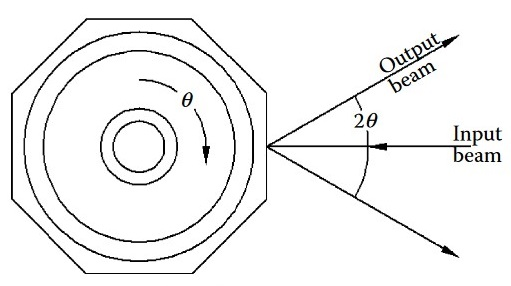
\includegraphics[width=0.5\textwidth]{img/polygon-scanner.jpg}
  \caption{\label{fig:polygon-scanner} mechanika polygonových skenerů}
\end{figure}

% \begin{figure}[!htb]
%   \centering
%   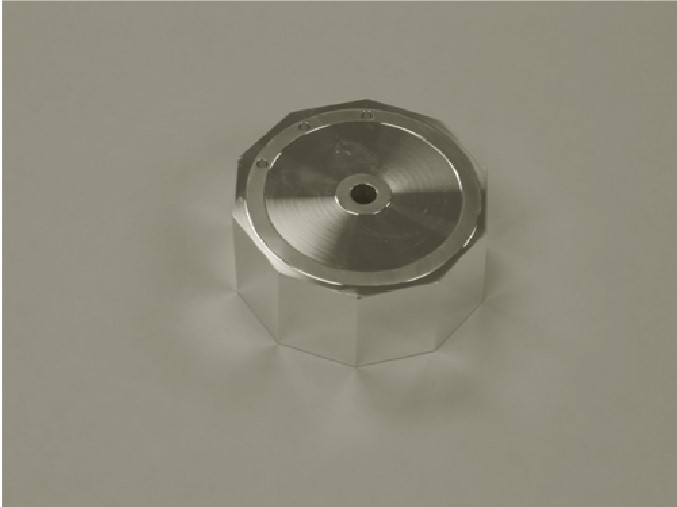
\includegraphics[width=0.5\textwidth]{img/polygon-prismatic-mirror.jpg}
%   \caption{\label{fig:polygon-prismatic-mirror} hranolové zrcátko polygonového skeneru}
% \end{figure}

% \begin{figure}[!htb]
%   \centering
%   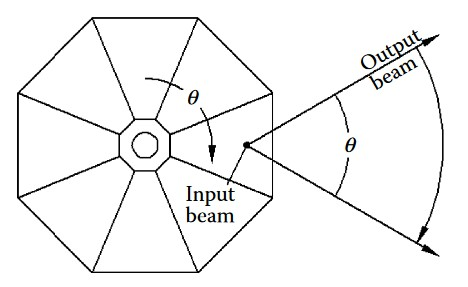
\includegraphics[width=0.5\textwidth]{img/polygon-pyramidal-mirror.jpg}
%   \caption{\label{fig:polygon-pyramidal-mirror} pyramidové zrcátko polygonového skeneru}
% \end{figure}
%

S jedním hranolem by hranolové skenery byly schopny směřovat paprsek pouze v jedné rovině - při projekci by bylo možné vykreslit maximálně čáru. Tuto limitaci lze kompenzovat přidáním melého rozdílu ve směřování každé strany hranolu, viz. obrázek \ref{fig:polygon-angular-variation}. S touto úpravou každá strana hranolu "vykreslí" jednu, svoji, přímku lehce posunutou vůči přímkách ostatních stran. Hranol s n-úhelníkovou podstavou je schopen vykreslit n přímek.
Další možností je kombinovat původní pravidelný hranol s galvanometrem (popsáno níže), kdy galvanometr nastaví jednu souřadnici paprsku a hranol na této souřadnici vykreslí přímku.

Tento typ skeneru se využívá hlavně pro senzory skenující na přímce (např. skenery čárových kódů~\cite{history-of-barcode-scanning}), nebo při rastrovém laser scanningu. Příklad rastrové projekce je vidět na obrázku \ref{fig:harddrive-projector-youtube}

\begin{figure}[!htb]
  \centering
  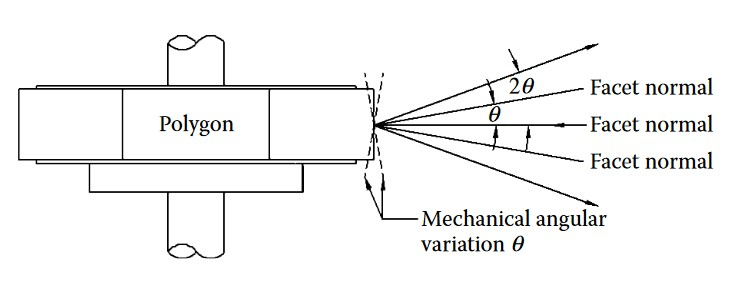
\includegraphics[width=0.8\textwidth]{img/polygon-angular-variation.jpg}
  \caption{\label{fig:polygon-angular-variation} úhlová rozdílnost polygonového skeneru}
\end{figure}


\begin{figure}[!htb]
  \centering
  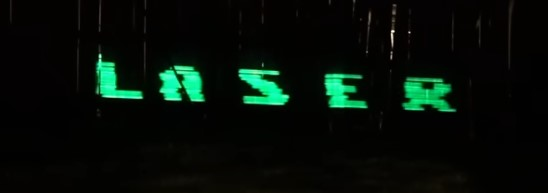
\includegraphics[width=0.5\textwidth]{img/harddrive-projection.jpg}
  \caption{\label{fig:harddrive-projection} příklad projekce laserového projektoru s polygonovým skenerem; zdroj \cite{harddrive-projector-youtube}}
\end{figure}

\section{Galvanometrové skenery}

Základní součástku galvanometrového skeneru je galvanometr.

\subsection{Galvanometr~\cite{some stuff}}      

\subsection{Konstrukce galvanometrových skenerů}
Jeden galvanometrový skener 

Narozdíl od hranolových skenerů je s galvanometrovým skenerem možné zastavit obě osy pohybu - vykreslovat na sebe kolmé čáry.

\begin{figure}[!htb]
  \centering
  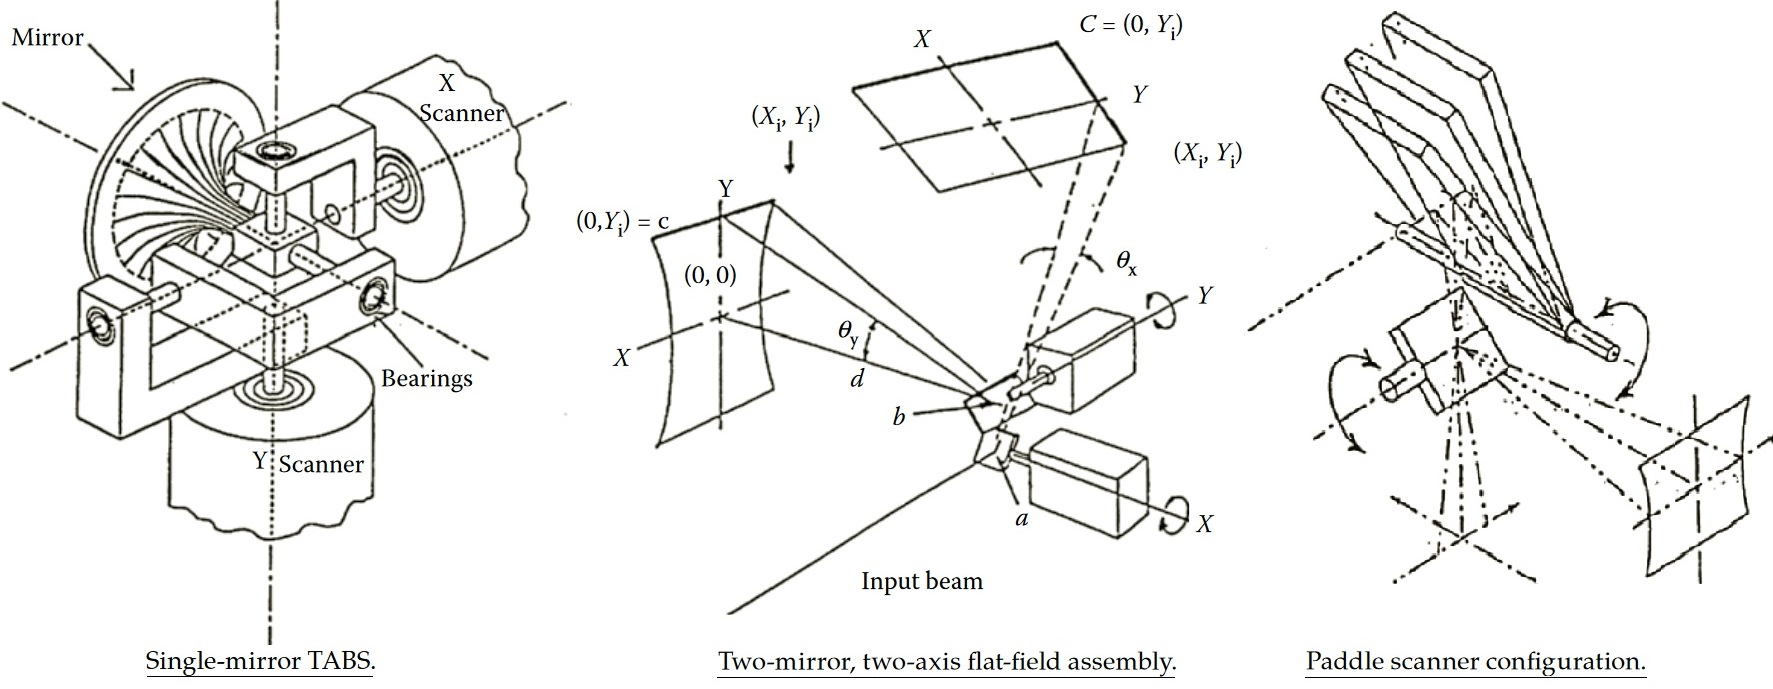
\includegraphics[width=1\textwidth]{img/scanner-constructions.jpg}
  \caption{\label{fig:scanner-constructions} různé konstrukce galvanometrových skenerů}
\end{figure}

\section{Má volba skeneru}

ja vyuzivam galva, protoze se s nima da nejlip pohrat, jsou nejuniverzalnejsi a tim padem nejvic zaujmou - cil